\chapter{State-of-the-Art} \label{chap:sota}

\section*{}

In this chapter we will begin by making a more in depth presentation of the
process of gene expression. This will be followed by a literature and state of
the art review in the fields of genome/\trans{} assembly and data mining.
Lastly, we will present some of the tools used in each of those areas, as well
as some relevant data representation formats for genetic data.

\section{Introduction}

Before dwelling in the details of the state of the art that are on the
foundation of this thesis, it is important to explain some concepts of the
domain of molecular biology. As explained in Section \ref{sec:context}, gene
expression is the mechanism by which an organism's \dna{} can be expressed into
functional genetic products, like proteins, rRNA and tRNA. This process starts
with the genetic code, or nucleotide sequence, of each gene. Different genes in
an organism's \dna{} are responsible for the creation of different genetic
products. The process of gene expression itself is composed by two main stages,
transcription and translation \cite{leic:gene_expr}.

Transcription is the stage at which genetic data in the form of \dna{} is used
to synthesize \rna{}, being this the process that concerns the thesis main
question. Several different types of \rna{} are produced by this process,
including mRNA (which specifies the sequences of amino acids that form a
protein), rRNA and tRNA, both later used in the translation stage. Simplifying a
gene's structure, it can be seen as composed by two types of areas, introns and
exons, as seen in Figure \ref{fig:intron_exon}.

\begin{figure}[!htb]
  \begin{center}
    \leavevmode
    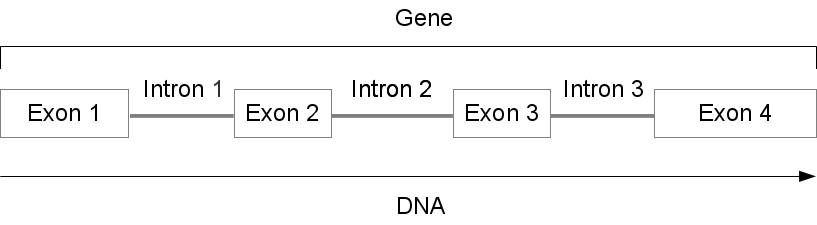
\includegraphics[width=0.7\textwidth]{intron_exon}
    \caption{Overall structure of a gene, with its different areas (simplified)}
    \label{fig:intron_exon}
  \end{center}
\end{figure}

Only the exons are useful in the gene expression process, being also known as
coding regions. Introns, on the other hand, are not used in the process. They
are present in an early stage mRNA molecule, the precursor RNA, but are later
removed (or spliced) in the final molecule before the translation stage
\cite{leic:gene_expr}. Figure \ref{fig:splicing} illustrates the removal of
introns from the mRNA molecule, during the  splicing process. As stated before,
the main goal of this thesis is to explain how the final nucleotide sequence of
each exon affects the transcription speed of the exon itself.

\begin{figure}[!htb]
  \begin{center}
    \leavevmode
    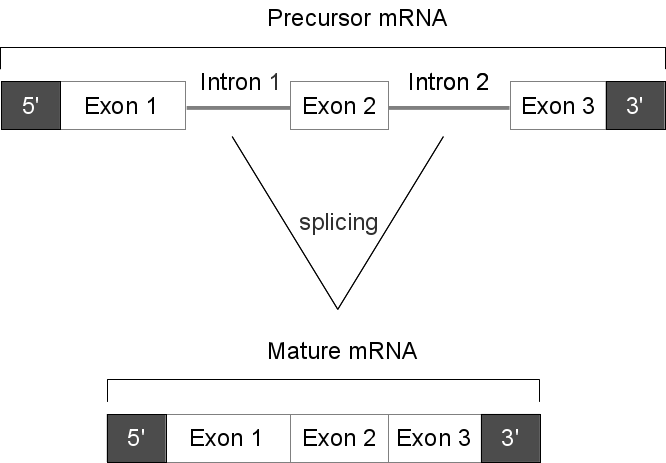
\includegraphics[width=0.58\textwidth]{splicing}
    \caption{The removal (splicing) of introns from the precursor mRNA, during
    the transcription process}
    \label{fig:splicing}
  \end{center}
\end{figure}

After the conclusion of the transcription process comes the translation process.
In this process, the synthesized mRNA is used to specify the sequence of amino
acids that constitute the particular protein being produced. The other types of
RNA molecules (rRNA and tRNA) are also used in this stage of the gene expression
process.

Obtaining this genetic information is done experimentally, by employing a genome
sequencing technique. For quite some time this process was carried out using the
Sanger sequencing method and other similar methods \cite{Reis-Filho2009}. Though
effective, such methods we're notably slow and costly, with large projects like
the Human Genome Project (HGP) consuming roughly thirteen years and US\$ 3
billion. The past few years have seen the appearance and rise in popularity of
the \ngs{} techniques. These techniques differ from the more classical ones by
producing larger amounts of information, in less time. They are also typically
more cost effective than previous techniques, which has greatly contributed to
their popularity. As a disadvantage, \ngs{} techniques produce shorter reads
than their older counterparts, posing a complicated problem in terms of genome
assembly and raising new computational challenges. Although this thesis will not
deal with the problems of sequencing techniques, it is important to indicate
that the read dataset that will be used is a result of \ngs{} techniques. As
such, we will use assembly techniques more suited to situations where short
reads are available.

\section{Genome Assembly and \rnaseq}\label{sec:assembly}

- talk about genome assembly, talk briefly about micro arrays, more about RNA
  seq and de novo vs guided assembly/alignment;\\

\subsection{\rnaseq{} Tools}\label{sec:seqtools}

\subsection{Relevant Standard File Formats}\label{sec:formats}

\section{Data Mining}\label{sec:mlearning}

\subsection{Data Mining Algorithms}\label{sec:minalgo}

\subsection{Data Mining Tools}\label{sec:mintools}

\section{Chapter Conclusions}
